\section{Lattice Vibrations \& Phonons}
\subsection{Phonons in One Dimension}
We consider a simple monoatomic chain:
\begin{figure}[htbp]
    \centering
    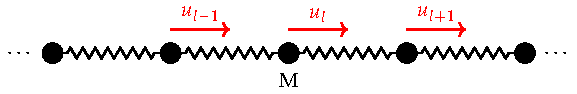
\includegraphics[]{Images/fig-monochaincartoon.pdf}

    \caption{A monoatomic chain. The atoms are of mass $M$ and are labelled with index $l$, with $u_l$ denoting the $l$th-atoms' displacement from equilibrium.}
    \label{fig-monochaincartoon}
\end{figure}
We label the atoms by index $l$ and the displacements from equilibrium for the $l$th atom by $u_l$. We assume we have a crystal lattice with individual atoms oscillating around equilibrium positions. The general Hamiltonian we can write for this system is:
\begin{equation}
    \begin{split}
        &H = \sum_l \frac{p_l^2}{2M} + V(u_1, u_2, \ldots)
        \\ &p_l = -i\hbar\dpd{}{u_l}
        \\ &[u_l, p_{l'}] = i\hbar\delta{ll'} 
    \end{split}
\end{equation}
Where we take the momentum to be canonically conjugate to the displacement and hence it satisfies the canonical commutation relation. We assume that the potential has a minimum for $u_l = 0$ for all $l$. We expand $V$ in a Taylor series about these minima:
\begin{equation}\label{eq-Vtaylor}
    V(u_1, u_2, \ldots) = V(0, 0, \ldots ) + \sum_l u_l \left[\dpd{V}{u_l}\right]_{u_1=u_2=\ldots = 0} + \frac{1}{2!}\sum_{l, l'}u_lu_{l'}\left[\frac{\partial^2 V}{\partial \mu_l \partial \mu_{l'}}\right]_{u_1=u_2=\ldots=0} + \frac{1}{3!} \ldots
\end{equation}
The first term can be eliminated by suitable choice of energy zero (a constant in the Hamiltonian changes none of the physics). The second term vanishes by virtue of $u_1 = u_2 = \ldots = 0$ being a minimum of $V$. We are left with just the second-order term, and so:
\begin{equation}
    H \approx \sum_l \frac{p_l^2}{2M} + \frac{1}{2}\sum_{l, l'}u_l V_{ll'}u_{l'}
\end{equation}
where $V_{ll'} = \left[\frac{\partial^2 V}{\partial \mu_l \partial \mu_{l'}}\right]_{u_1=u_2=\ldots=0}$ is the dynamical matrix. We neglect all higher order terms in Eq. \eqref{eq-Vtaylor} which amounts to a harmonic approximation.

\subsection{Diagonalizing the Potential}

We next diagonalize the $V$-term. To this end, we define a vector of displacements:
\begin{align*}
    Y = \m{\mu_1 \\ \mu_2 \\ \vdots \\}
\end{align*}
and then we have:
\begin{align*}
    V = \m{V_{11} & V_{12} & \ldots
    \\ V_{21} & \ddots & 
    \\ \vdots & &}
\end{align*}

We now write that the $V$-term is:
\begin{equation}
    Y^T V Y = Y^T U^\dag U V U^\dag U Y = (Y^T U^\dag) (U V U^\dag) (U Y) = \tilde{Y}^\dag \tilde{V} \tilde{Y} = \sum_q \tilde{Y}_q^\dag \tilde{V}_{qq}\tilde{Y}_q
\end{equation}
where $U$ is the unitary matrix that diagonalizes $V$. This is of course nothing more than a change of basis. Since it is diagonal in the new basis, we can index it with a new index $q$.

It is easy to see that this transformation leaves the kinetic energy unchanged (i.e. it remains diagonal!). To this end we consdier:
\begin{equation}
    p_l = -i\hbar\dpd{}{\mu_l} = -i\hbar \sum_q \dpd{\tilde{\mu}_q}{\mu_l}\dpd{}{\tilde{\mu}_q} = -i\hbar \sum_q U_{lq}\dpd{}{\tilde{\mu}_q} = \sum_q U_{lq} (-i\hbar\dpd{}{\tilde{\mu}_q})
\end{equation}
or in other words: $\tilde{P} = U^{-1}P$. Therefore:
\begin{equation}
    \sum p_l^2 = P^TP = (U\tilde{P})^\dag(U\tilde{P}) = \tilde{P}^\dag U^\dag U \tilde{P} = \tilde{P}^\dag \mathbb{I} \tilde{P} = \tilde{P}^\dag \tilde{P} = \sum_q \tilde{p}_q^\dag \tilde{p}_q
\end{equation}
So the kinetic energy remains diagonal! An important remark; in our canonical representation, $P$ is a Hermitian operator. But the transformed $P$ may no longer have this property, so we keep the $\tilde{p}_q^\dag$ in the last expression (instead of assuming it will be equal to $\tilde{p}_q$). In the new coordinates, the Hamiltonian reads:
\begin{equation}\label{eq-diagonalizedlatticeH}
    H = \sum_q \left(\frac{1}{2M}p^\dag_q p_q + \frac{1}{2}M\omega_q\mu^\dag_q \mu_q\right)
\end{equation}
where we define $\omega_q^2 = V_q/M$ (and dropped the $\sim$s so we don't have to keep writing it; the new coordinates are distinguished via their index). So our $H$ is diagonal! Let us also note that the unitary transformation preserves the commutation rules (Check!), so:
\begin{equation}
    [\mu_q, p_{q'}] = i\hbar\delta_{qq'}.
\end{equation}

Eq. \eqref{eq-diagonalizedlatticeH} is seen to describe a collection of decoupled harmonic oscillators; we can solve this by the usual raising and lowering operator method. For each mode we define:
\begin{equation}\label{eq-raisinglowering}
    \begin{split}
        a_q &= \frac{1}{\sqrt{2M\hbar \omega_q}}\left(M\omega_q \mu_q + ip_q^\dag\right)
        \\ a_q^\dag &= \frac{1}{\sqrt{2M\hbar \omega_q}}\left(M\omega_q \mu_q^\dag - ip_q\right)
    \end{split}
\end{equation}
these satisfy the usual algebra of raising and lowering operators:
\begin{align*}
    [a_q, a_q^\dag] = \delta_{qq'}.
\end{align*}
In this representation the Hamiltonian acquires a simple form:
\begin{equation}
    H = \sum_q \hbar \omega_q\left(a^\dag_q a_q + \frac{1}{2}\right)
\end{equation}
Often the goal is to know what the $\omega_q$ is; this will give us the spectrum of excitations and how they depend on $q$. We will comment on this shortly when we do an example. In principle this is not difficult as $\omega_q = V_q/M$, and we can get $V_q$ from transforming the dynamical matrix. 

\subsection{Translation-Invariant Systems}
This entire discussion so far was quite general; however since most solid-state systems are translation invariant, we can now consider such systems to analyze. In particular, this has the effect that the dynamical matrix depends only on differences $l - l'$:
\begin{equation}
    V_{ll'} = V_{l-l'}
\end{equation}
This is useful as we can guess immediately what the transformation will be; a Fourier transform!
\begin{equation}
    U_{ql} = \frac{1}{\sqrt{N}}e^{iql}
\end{equation}
therefore:
\begin{equation}
    \tilde{V}_{qq'} = [U^\dag VU]_{qq'} = \frac{1}{N}\sum_{ll'}e^{-iql}V_{l-l'}e^{iql'} = \left(\frac{1}{N}\sum_{l'}e^{-il'(q-q')}\right)\left(\sum_{l}e^{-iql}V_l\right) = \delta_{qq'}V_q
\end{equation}
where in the third equality we make the substitution $l \to l + l'$. In the fourth equality the $\delta$ comes from basic Fourier analysis (one can imagine the oscillations exactly cancelling if $q \neq q'$, and exactly adding up if $q = q'$).

We will now see what are the consequences we can draw from this. One thing to specify before we go on: let us use periodic boundary conditions, so that the last atom in the chain of atoms is connected back to the first chain. Mathematically, this is expressed as:
\begin{align*}
    \mu_{l + Na} = \mu_l
\end{align*}
where in the above $l$ represents a distance rather than an index. Note that this implies $e^{iql} = e^{iq(l+Na)}$. This further implies a restriction on the form of the $q$s, namely:
\begin{equation}
    1 = e^{iqNa} \implies q = \frac{2\pi n}{Na}, \quad n \in \ZZ.
\end{equation}
From this we have:
\begin{equation}
    \mu_q = \frac{1}{\sqrt{N}}\sum_l e^{-iql}\mu_l, \quad p_q = \frac{1}{\sqrt{N}}\sum_l e^{iql}p_l
\end{equation}
It follows that:
\begin{equation}
    \mu_{q + G} = \mu_q, \quad p_{q + G} = p_q, \text{ with } G = \frac{2\pi}{a}.
\end{equation}
Therefore; momentum is only defined in the ``1st Brillouin zone'' with $q \in (-\frac{\pi}{a}, \frac{\pi}{a})$ and there are only $N$ distinct values,
\begin{equation}
    q = \frac{2\pi n}{Na}, \quad  n = -\frac{N}{2} + 1, \ldots \frac{N}{2}.
\end{equation}

Much like the case with electrons in a periodic potential, for phonons everything happens in the first Brillouin zone. 

One more comment before proceeding with an example. It also holds that:
\begin{align*}
    \mu_q^\dag = \mu_{-q}, \quad p_q^\dag = p_{-q}
\end{align*}
further accenting that the transformed $\mu/p$s are not Hermitian, unlike their canonical counterparts? Taking into account $\omega_{-q} = \omega_q$, Eqs. \eqref{eq-raisinglowering} can be inverted as:
\begin{equation}
    \begin{split}
        \mu_q = \sqrt{\frac{\hbar}{2M\omega_q}}(a^\dag_{-q} + a_q)
        \\ p_q = i\sqrt{\frac{M\hbar \omega_q}{2}}(a^\dag_{-q} - a_q)
    \end{split}
\end{equation}
This is not profound (it is just an inversion) but will be quite useful when we proceed to calculate expectation values of operators.

\subsection{Example 1 - Monoatomic chain}
We consider again a monoatomic chain as in Fig. \ref{fig-monochaincartoon}; a system of masses $M$ connected by springs of spring constant $K$ with periodic boundary conditions. The potential energy (and from it the dynamical matrix) is given by:
\begin{equation}
    \begin{split}
        V &= \sum_l \frac{1}{2}K(\mu_{l} - \mu_{l+1})^2 = \sum_l \frac{1}{2}K\left(2u_l^2 - 2u_lu_{l+1}\right)
        \\ \implies  V_{ll'} &= \begin{cases}
            2K & \text{if $l = l'$}
            \\ -K & \text{if $l = l' \pm 1$}
            \\ 0 & \text{otherwise}
        \end{cases}
    \end{split}
\end{equation}
note there is no factor of $2$ in front of the $-K$ because there are two entries in the matrix; one above/below the diagonal. The fourier transform gives:
\begin{equation}
    V_q = 2K - K(e^{iqa} + e^{-iqa}) = 2K(1 - \cos(qa)) = 4K\sin^2\frac{qa}{2}
\end{equation}
from this we can read off the spectrum of normal modes:
\begin{equation}
    \omega_q = \sqrt{\frac{V_q}{M}} = 2\sqrt{\frac{K}{M}}\abs{\sin\frac{qa}{2}} \approx \sqrt{\frac{K}{M}}\abs{qa} \text{ for $\abs{qa} \ll 1$}
\end{equation}
so the dispersion is linear (for small $qa$), signifying a sound-like or acoustic mode. This should be true, because sound propogates through solids! Let us now sketch the spectrum, as a function of $q$; known as the ``phonon dispersion'' of the ``phonon energy spectrum''. We often focus on a phonon of a particular wavenumber $q$ and specific energy; and this is indeed something that is experimentally measurable! (E.g. by neutron scattering).

\begin{figure}[htbp]
    \centering
    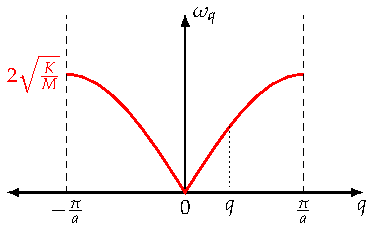
\includegraphics[]{Images/fig-monochaindispersion.pdf}
    \caption{Dispersion relation for the monoatomic chain.}
    \label{fig-monochaindispersion}
\end{figure}

\newpage 
\subsection{Example 2 - Diatomic Chain}

\begin{figure}[htbp]
    \centering
    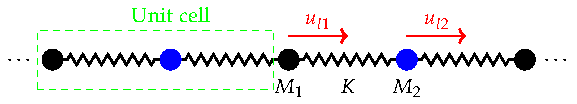
\includegraphics[]{Images/fig-diachaincartoon.pdf}
    
    \caption{A diatomic chain. We have alternating atoms of mass $M_1/M_2$ joined by springs of spring constant $K$. We index the displacement of the $M_1$ atoms with $u_{l_1}$ and the $M_2$ atoms as $u_{l_2}$. A unit cell contains one atom of each type and two springs.}
    \label{fig-diachaincartoon}
\end{figure}
We now consider a diatomic chain. We now have two different types of atoms in our chain; mass $M_1$ and mass $M_2$. The springs between them are still of spring constant $K$. The unit cell contains one atom of each type and two of the springs. We denote the displacement of the $M_1$ atoms as $u_{l_1}$ and the $M_2$ atoms as $u_{l_2}$.



Similar analysis as before gives the momentum space dynamical matrix (Check!):
\begin{equation}
    V_q = \m{2K & -K(1-e^{iqa}) \\ -K(1+e^{-iqa}) & 2K}
\end{equation}
The Hamiltonian that follows from this is:
\begin{equation}
    H = \sum_q \left(\frac{p_{q_1}^\dag p_{q_1}}{2M_1} + \frac{p_{q_2}^\dag p_{q_2}}{2M_2}\right) + \frac{1}{2}\sum_{q}\m{\mu_{q_1}^\dag & \mu_{q_2}^\dag} V_{q}\m{\mu_{q_1} \\ \mu_{q_2}}
\end{equation}
this is typical for a more complicated chain, where $N$ different atoms would give an $N \times N$ $V_q$ matrix in momentum space. Another complication is that $M_1 \neq M_2$, and so it is not immediate to read off $\omega_q$; we need to get rid of unequal masses in the kinetic energy term. This is done through the rescaling of momenta:
\begin{equation}
    p_{q_1} \to p_{q_1}\left(\frac{M_1}{M_2}\right)^{1/4} \quad p_{q_2} \to p_{q_2}\left(\frac{M_2}{M_1}\right)^{1/4}
\end{equation}
This implies a corresponding scaling of the displacements:
\begin{equation}
    \mu_{q_1} \to \mu_{q_1}\left(\frac{M_2}{M_1}\right)^{1/4} \quad \mu_{q_2} \to \mu_{q_2}\left(\frac{M_1}{M_2}\right)^{1/4}
\end{equation}
so the Hamiltonian becomes:
\begin{equation}
    H = \sum_q \frac{p_{1q}^\dag p_{1q} + p_{2q}^\dag p_{2q}}{2\sqrt{M_1M_2}} + \frac{1}{2}\sum_q \m{\mu_{q_1}^\dag & \mu_{q_2}^\dag} \m{2K\sqrt{\frac{M_1}{M_2}} & -K(1+e^{iqa}) \\ -K(1+e^{-iqa}) & 2K\sqrt{\frac{M_2}{M_1}}}\m{\mu_{q_1} \\ \mu_{q_2}}
\end{equation}
the normal modes are given by eigenvalues of $\tilde{V}_q$ (the matrix in the potential energy term above):
\begin{equation}
    0 = \det(\tilde{V}_q - \omega\sqrt{M_1M_2}) = M_1M_2\omega^4 - 2K(M_1+ M_2)\omega^2 + 2K^2(1-\cos qa)
\end{equation}
This is just a quadratic equation in $\omega^2$, so:
\begin{equation}
    \omega_{12}^2 = \frac{2K}{M_1M_2}\left((M_1 + M_2) \pm \sqrt{(M_1 + M_2)^2 - 2M_1M_2(1 - \cos qa)}\right)
\end{equation}
If we sketch the dispersion realtion, we have:

\begin{figure}[htbp]
    \centering
    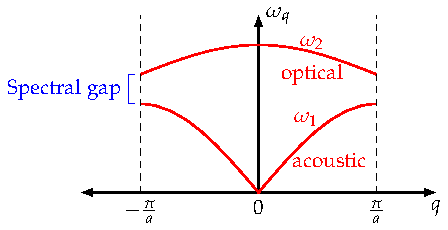
\includegraphics[]{Images/dig-diachaindispersion.pdf}

    \caption{Dispersion relations for diatomic chain. Note the presence of two different branches/phonon modes, and the spectral gap between them.}
    \label{fig-diachaindispersion}
\end{figure}

The acoustic branch is linear and the basis of sound waves inside of the material. The optical branch is excited by shining light on the material. If we shine waves of an intermediate energy in the spectral gap (in between hte two branches), none will propagate!

Next class, we will discuss phonons further; in particular how they behave in 3D, and thermodynamic properties of vibrating crystals.